\documentclass[a4paper,10pt]{article}
\usepackage[left=1in,right=1in,top=1in,bottom=1in]{geometry}
\usepackage{graphicx}
\usepackage{subcaption}
\usepackage{hyperref} % Pour rendre les sections de la table des matières cliquables
\usepackage[french]{babel} % Pour que la date soit en français
\usepackage{float} 
\usepackage[utf8]{inputenc}
\usepackage[T1]{fontenc}
\usepackage{fancyhdr}
\usepackage{lipsum}

% Définition du logo
\newcommand{\logo}{
\includegraphics[width=5cm]{captures/unicaen.png}}

% Définition du style de page avec le logo
\fancypagestyle{mylogo}{
    \fancyhf{}
    \fancyhead[R]{\logo} % Logo en haut à droite
    \renewcommand{\headrulewidth}{0pt}
}


% Titre du projet et noms des contributeurs

\newcommand{\projet}{\vspace{10cm} Jeu de Puzzle à glissières (Taquin)}
\newcommand{\contributeurs}{\textbf{ABDULRAZAK} Tariq, \textbf{KAMGANG KENMOE} Miguel Jordan, \textbf{DIALLO} Mariatou , }
\newcommand{\contributeurss}{\textbf{ABOGOUNRIN} Ayath}
\newcommand{\chargeTP}{\textbf{Yann MATHET}}

\title{\projet}
\author{\contributeurs \\ \contributeurss \\ \\ Responsable de TP : \chargeTP}
\date{\today}


\begin{document}

\maketitle
\thispagestyle{mylogo} 

\newpage
\tableofcontents
\clearpage

\section{Introduction}

\subsection{Présentation du projet}
Le jeu de puzzle à glissières, également connu sous le nom de Taquin, est un casse-tête
classique qui met à l'épreuve la réflexion et la logique des joueurs. Créé à l'origine au 18e
siècle, ce jeu simple mais captivant a été adapté dans de nombreuses versions à travers les
âges, allant des versions physiques aux applications mobiles et aux jeux en ligne.\\ \\
Cette version informatisée du jeu de puzzle à glissières propose une approche interactive et
dynamique du Taquin, permettant aux joueurs de résoudre le casse-tête sur leur ordinateur.
Avec des fonctionnalités telles que le redimensionnement automatique de la grille,
le suivi du nombre de mouvements effectués et la détection de la fin du jeu,
cette application offre une expérience de jeu engageante et stimulante.\\ \\
Dans ce rapport, nous explorerons les aspects techniques de l'implémentation de cette version du
jeu de puzzle à glissières,
en mettant en lumière les concepts de programmation utilisés pour créer une interface
utilisateur interactive et intuitive.

\subsection{Objectifs du projet}
Le projet avait plusieurs objectifs clés. Tout d'abord, nous souhaitions concevoir une interface utilisateur intuitive et facile à utiliser qui permettrait aux utilisateurs de jouer sans difficulté. Mais tout cela en gardant le principe de MVC (Modèle-Vue-Contrôleur), autrement dit, notre jeu reste complètement jouable en ligne de commande et le fait d'ajouter une interface graphique ne change absolument rien à notre code du modèle. Nous avons également cherché à généraliser le plus possible, c'est-à-dire que notre code marche pour n'importe quelle taille de grille (tant qu'elle est carrée). Enfin, nous avons cherché à concevoir l'application de manière à ce qu'elle soit extensible et facile à maintenir, de sorte que des améliorations puissent être apportées à l'avenir sans avoir à repenser complètement le code.

notre objectif est de réaliser ce jeu en Console et en Graphique comme la suite : 

\begin{figure}[H]
\centering
\begin{subfigure}{0.50\textwidth}
  \centering
  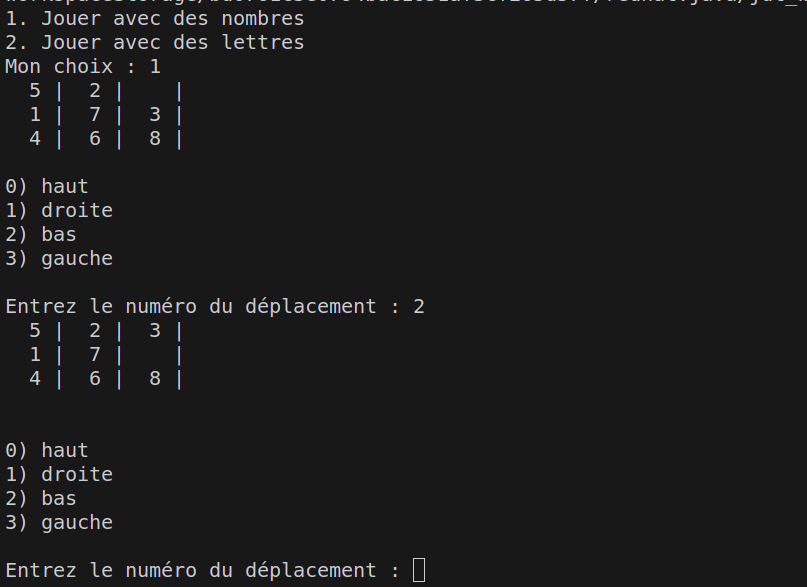
\includegraphics[width=\linewidth]{captures/consol.png}
  \caption{Grille de nombres en Console}
\end{subfigure}
\hfill
\begin{subfigure}{0.45\textwidth}
  \centering
  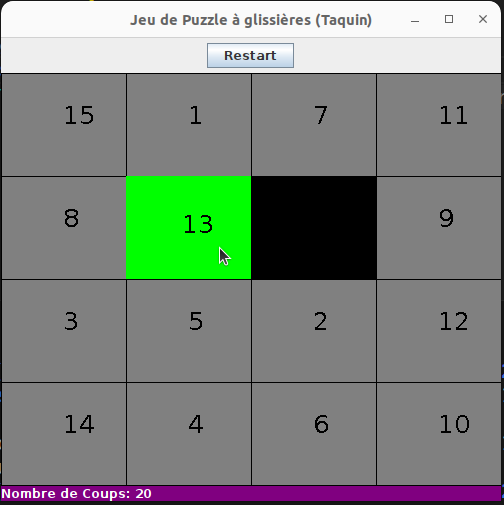
\includegraphics[width=\linewidth]{captures/image.png}
  \caption{Grille de nombres en graphic}
\end{subfigure}
\end{figure}

\subsection{Contexte}
Le projet a été réalisé dans le cadre de 4 cours d'interface graphique, qui visaient à nous donner une expérience pratique de la conception et du développement de logiciels en équipe. Nous avons travaillé ensemble pour identifier les exigences du projet, élaborer un plan de travail et mettre en œuvre des solutions techniques pour surmonter les défis rencontrés tout au long du développement.

Au-delà de la simple programmation, le projet nous a permis de développer nos compétences en matière de gestion de projet, de communication d'équipe et de résolution de problèmes. Nous avons travaillé en étroite collaboration pour nous assurer que le développement se déroule sans accroc et que l'application soit livrée à temps pour la date limite fixée le 15 avril 2024 à 17h .


\section{Description}

\subsection{Règles du jeu}
Le jeu de puzzle à glissières, également connu sous le nom de Taquin, propose un défi captivant où les joueurs doivent réorganiser des pièces désordonnées pour former une image ou une séquence numérique correcte. En déplaçant les pièces adjacentes à une case vide, les joueurs doivent trouver la bonne séquence de mouvements pour résoudre le puzzle. Avec différentes variations de puzzles disponibles, le jeu offre une expérience stimulante adaptée à tous les niveaux de compétence. La résolution réussie du puzzle est marquée par l'alignement correct de toutes les pièces.

\subsection{Spécificités du jeu de puzzle à glissières}

Notre version du jeu de puzzle à glissières, inspirée du classique Taquin, offre une expérience unique grâce à ses règles spécifiques :

\begin{itemize}
\item \textbf{Taille de la grille personnalisable :} Contrairement aux versions traditionnelles qui proposent souvent des grilles de taille fixe, notre jeu permet aux joueurs de choisir la taille de la grille selon leurs préférences. Cela offre une flexibilité et une variété supplémentaires dans le défi proposé.

\item \textbf{Déplacement interactif des pièces :} Afin de rendre le jeu plus engageant et immersif, nous avons inclus une fonctionnalité permettant aux joueurs de déplacer les pièces de manière interactive. Lorsqu'une pièce est sélectionnée, elle clignote avec une couleur distinctive, ce qui permet aux joueurs de visualiser clairement les mouvements possibles.

\item \textbf{Fonction de redémarrage :} Notre jeu est doté d'une fonction de redémarrage pratique qui permet aux joueurs de réinitialiser la grille à son état initial à tout moment. Cette fonctionnalité est utile pour les joueurs qui souhaitent recommencer le jeu à partir de zéro, corriger des erreurs ou relever à nouveau le défi avec une nouvelle approche.

\item \textbf{Calcul du nombre de coups :} Dans notre jeu, le nombre de coups est calculé de manière dynamique tout au long de la partie.
\end{itemize}

\section{Conception du projet}

\subsection{Analyse des besoins}
Avant de commencer à concevoir l'application, nous avons d'abord effectué une analyse approfondie des exigences du projet. Nous avons identifié les fonctionnalités clés dont l'application avait besoin, telles que un projet 100\% MVC avec d'abord un jeu sans interface graphique, puis l'ajout de l'interface graphique sans changer le code de notre jeu.

Nous avons également pris en compte les contraintes techniques du projet, notamment les langages de programmation et les outils disponibles pour développer l'application, ainsi que les délais impartis pour le développement et la livraison de l'application.

\subsection{Choix des technologies}
Nous devions utiliser le langage de programmation Java pour développer l'application. Nous avons également utilisé la bibliothèque graphique Swing pour la conception de l'interface utilisateur, car elle offre une grande flexibilité et est facile à utiliser.

Nous avons principalement utilisé VSCode comme éditeur, car nous avons trouvé qu'il était plus utile pour nous en tant qu'étudiants, surtout que les éditeurs comme Eclipse font une bonne partie du travail à notre place.

Nous avons utilisé Git pour le contrôle de version du code source et la forge pour héberger le
projet et faciliter la collaboration entre les membres de l'équipe.

\subsection{Architecture du projet}

Nous avons conçu l'application en utilisant une architecture de modèle-vue-contrôleur (MVC).
Cette architecture permet de séparer la logique métier de la présentation de l'interface
utilisateur, ce qui facilite la maintenance du code et permet d'ajouter de nouvelles
fonctionnalités plus facilement à l'avenir.

Le modèle représentait l'état actuel du jeu, y compris la grille, les coups joués et un bouton
Restart.
 Le contrôleur était responsable de la gestion des actions des utilisateurs, comme les coups joués, tandis que la vue représentait l'interface utilisateur de l'application.

\begin{figure}[H]
\begin{subfigure}{1.2\textwidth}
  \centering
  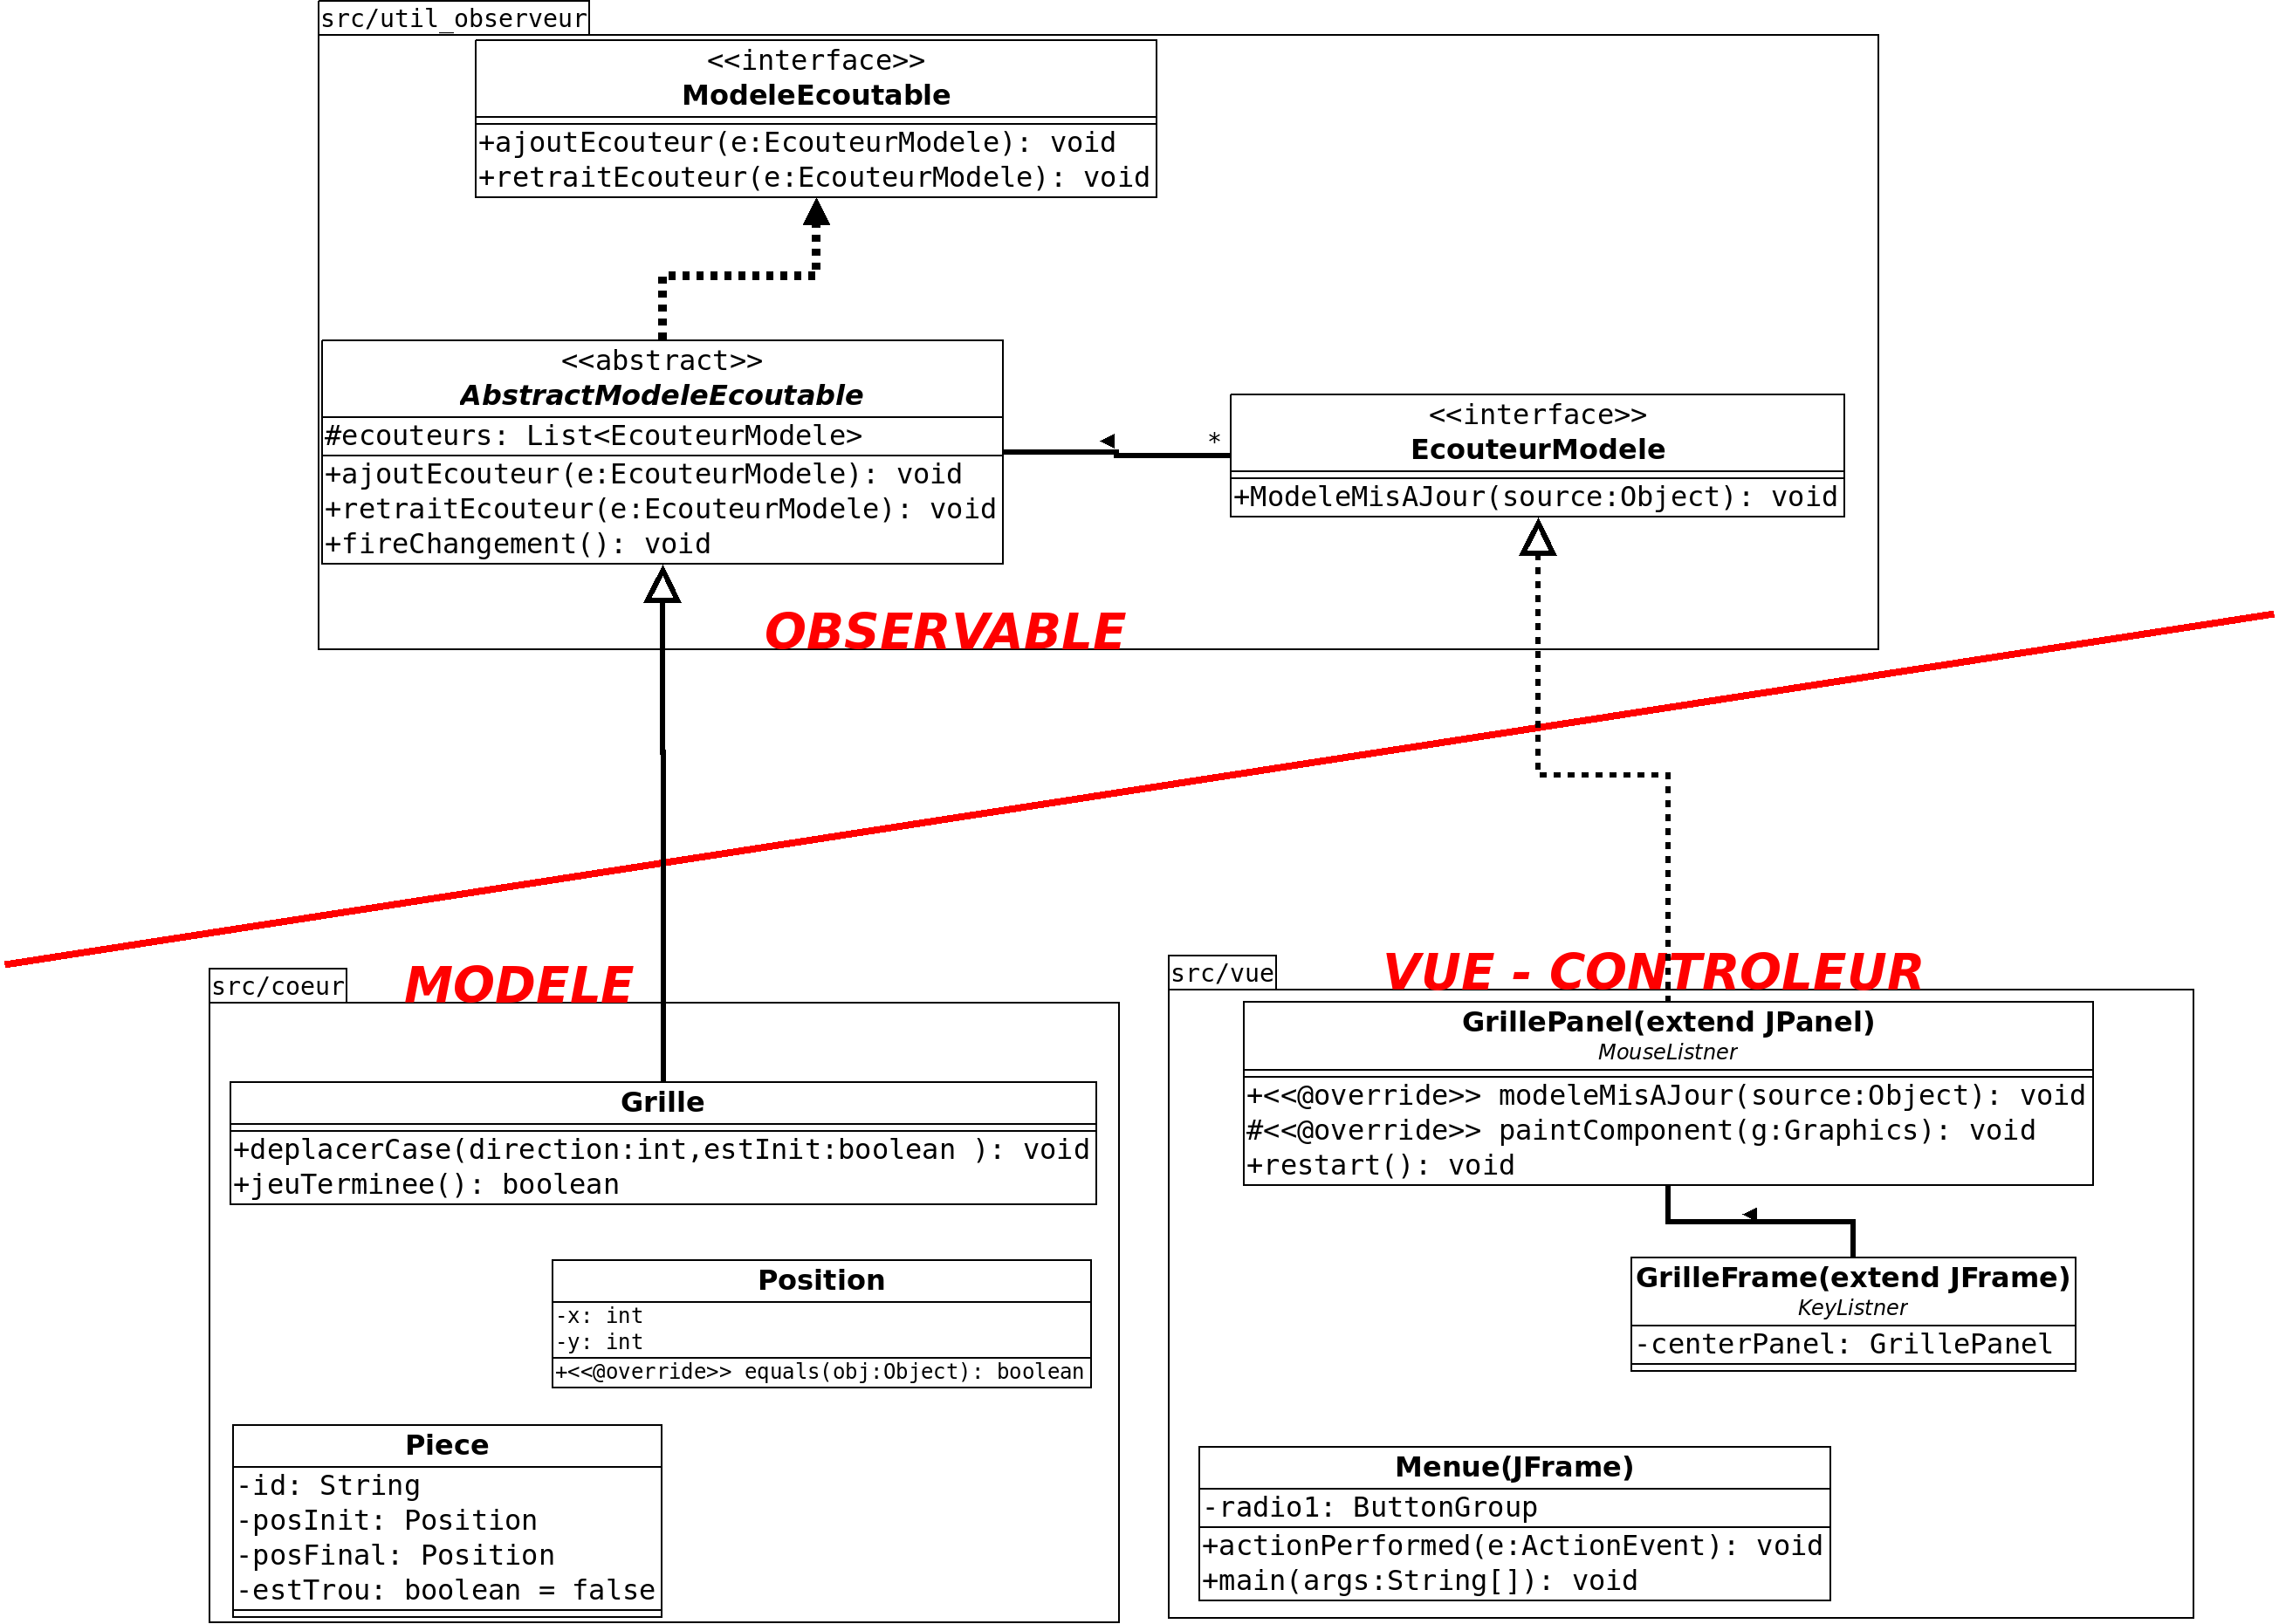
\includegraphics[width=\linewidth]{captures/Dia.png}
  \caption{Diagramme de classe MVC}
\end{subfigure}

\end{figure}


Pour la construction MVC, nous avons une classe abstraite \textbf{AbstractModeleEcoutable} qui représente tous les modèles que l'on peut écouter. Cette classe possède trois méthodes, deux pour ajouter ou retirer un \textbf{EcouteurModele} et la dernière pour avertir tous les \textbf{EcouteurModele} que le modèle a changé. Notre classe \textbf{Grille} hérite d'\textbf{AbstractModeleEcoutable}, donc elle possède la méthode \textbf{fireChangement()} qu'on appelle à chaque tour de boucle de jeu.

D'autre part, l'interface \textbf{EcouteurModele} représente toutes les vues, autrement dit, toutes les classes qui peuvent écouter une autre classe. Cette interface possède une méthode abstraite \textbf{ModeleMiseAJour()} qui est appelée chaque fois que le modèle appelle la méthode \textbf{fireChangement()}. Cette méthode \textbf{ModeleMiseAJour()} dit à notre affichage qu'il doit se mettre à jour car le modèle a changé.

\subsection{Les packages}
Nous avons séparé le code en plusieurs packages et voici leurs utilités :

\begin{itemize}
\item \textbf{util-observeur} : Ce package contient tous les patrons observateurs (observables).

\item \textbf{coeur} : Ce package contient les bases de notre jeu, c'est le cœur du jeu, il contient les classes (Grille, Piece, Position, ConsoleGrille et Main).

\item \textbf{Vue} : Ce package contient tout ce qui est lié à la partie graphique de notre projet, c'est-à-dire (Menu, GrilleFrame et GrillePanel).
\end{itemize}

\subsection{Partie graphique}

\textbf{Dans l'interface graphique, le contrôle sera fait de deux façons simultanées :} \\

\begin{itemize}

\item Un clic sur l'élément que l'on souhait déplacer (s'il est déplaçable). Un plus sera de mettre enexergue (par exemple en l'encadrant) un élément survolé par la souris lorsque celui-ci est déplaçable, ce qui permet à l'utilisateur de mieux voir ce qu'il peut faire.

\item Dans l'interface graphique, le contrôle sera fait de deux façons simultanées :

\item un clic sur l'élément que l'on souhait déplacer (s'il est déplaçable). Un appui sur 4

\end{itemize} 

\vspace{0.5cm}
Pour factoriser au mieux le code des grilles, nous avons décidé d'avoir la vue et les contrôleurs dans un seul package. \\ \\
Nous avons la classe Menu qui représente notre Menu et qui contient des choix pour l'utilisateur entre jouer avec une grille de nombres ou de lettres.

\begin{figure}[H]
\centering
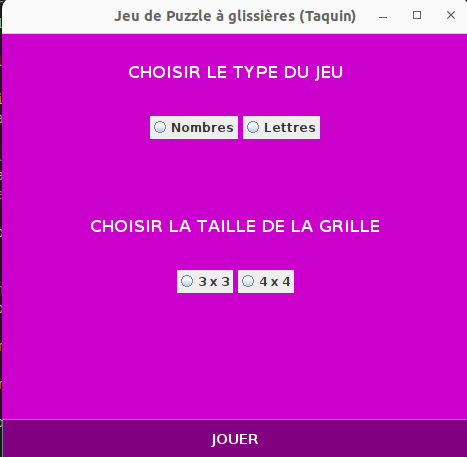
\includegraphics[scale=0.6]{captures/menu.png}
\caption{Menu de notre jeu}
\end{figure}

Ensuite, nous avons les deux classes GrilleFrame et GrillePanel.

La classe GrilleFrame représente la fenêtre principale du jeu. Elle est responsable de la disposition des éléments graphiques et de la gestion des interactions avec l'utilisateur. Voici une explication détaillée de ses fonctionnalités :

\begin{itemize}
\item \textbf{Création de la fenêtre :} La fenêtre est créée avec un titre spécifique et une taille prédéfinie.
\item \textbf{Disposition des éléments :} Les éléments graphiques tels que la grille de jeu et les boutons sont disposés à l'intérieur de la fenêtre selon un agencement spécifié.
\item \textbf{Gestion des interactions :} Les actions de l'utilisateur, telles que le redimensionnement de la grille et le clic sur les boutons, sont gérées par des écouteurs d'événements associés à chaque composant.
\item \textbf{Lancement du jeu :} Lorsque l'utilisateur clique sur le bouton "Jouer", une nouvelle instance de la classe GrilleFrame est créée pour démarrer le jeu.
\end{itemize}

La classe GrillePanel représente le panneau contenant la grille de jeu. Elle est responsable de l'affichage de la grille et de la gestion des interactions avec l'utilisateur.

\begin{itemize}
\item \textbf{Initialisation de la grille :} Une instance de la classe Grille est créée avec les dimensions spécifiées et le type de jeu (nombres ou lettres).
\end{itemize}



\begin{figure}[H]
\centering
\begin{subfigure}{0.45\textwidth}
  \centering
  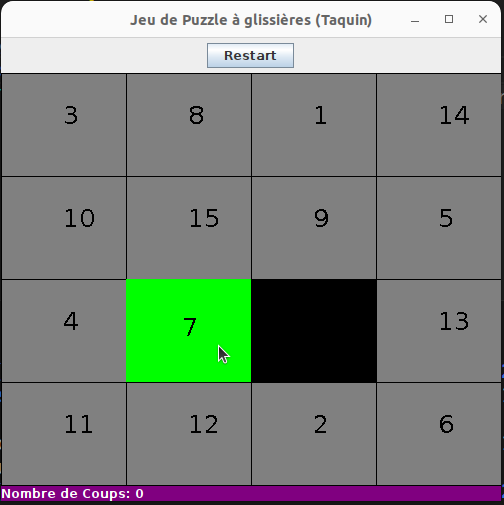
\includegraphics[width=\linewidth]{captures/colorer.png}
  \caption{Grille de nombres}
\end{subfigure}
\hfill
\begin{subfigure}{0.45\textwidth}
  \centering
  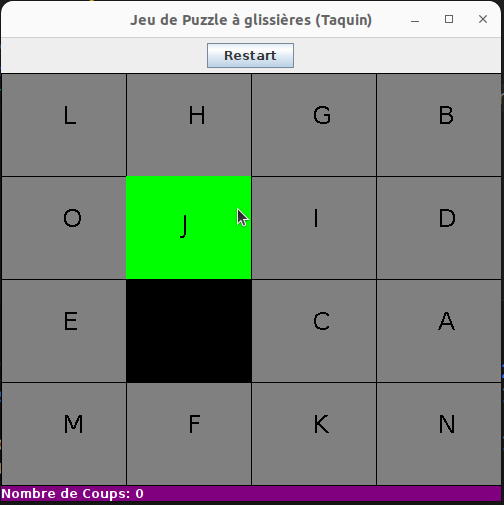
\includegraphics[width=\linewidth]{captures/lettres.png}
  \caption{Grille de lettres}
\end{subfigure}
\caption{Grilles de nombres et de lettres}
\end{figure}

\vspace{2cm}

Et pour l'affichage quand on finit de résoudre notre magnifique puzzle de taquin on aura un petit message qui indique qu'on a gagné la partie le trou devient une pièce visible et en même temps on affiche le nombre de coups effectué :)


\begin{figure}[H]
\centering
\includegraphics[scale=0.6]{captures/VersionFinal.png}
\caption{Version finale de notre jeu}
\end{figure}


\section{Conclusion}

\subsection{Résumé du projet}
Dans l'ensemble, le jeu de puzzle à glissières en Java a été un succès. Nous avons réussi à concevoir et à développer une application fonctionnelle qui permet aux utilisateurs de jouer. Nous avons également travaillé en étroite collaboration pour gérer le projet et surmonter les défis rencontrés tout au long du développement.
\subsection{Perspectives d'amélioration}
Cependant, il y a toujours des perspectives d'amélioration pour notre application. Par exemple :

\begin{enumerate}
    \item Mettre en place un mode multijoueur où deux grilles sont affichées et deux utilisateurs peuvent jouer simultanément. Le premier joueur à terminer sa grille remporte la partie.
    
    \item Ajouter une option pour jouer avec des images plutôt qu'avec des nombres ou des lettres, ce qui rendrait le jeu plus visuellement attractif.
    
    \item Implémenter une interface graphique plus conviviale pour afficher les résultats à la fin du jeu, au lieu de simplement afficher du texte. Cela pourrait inclure des animations, des graphiques ou d'autres éléments visuels pour rendre l'expérience plus engageante.
\end{enumerate}

\end{document}